\documentclass[12pt,a4paper]{article}

% Pachete pentru limba romana si fonturi
\usepackage[utf8]{inputenc}
\usepackage[T1]{fontenc}
\usepackage[romanian]{babel}
\usepackage{mathptmx} % Times New Roman
\usepackage{setspace}
\setstretch{1.15}

% Setari pagina
\usepackage[top=2.5cm, bottom=2.5cm, left=2.5cm, right=2cm]{geometry}
\usepackage{graphicx}
\usepackage{amsmath}
\usepackage{amssymb}
\usepackage{hyperref}
\usepackage{float}
\usepackage{enumitem}
\usepackage{indentfirst} % Alineat si la primul paragraf dupa titlu
\usepackage{array}
\usepackage{booktabs}
\usepackage{caption}
\usepackage{tikz}
\usetikzlibrary{shapes.geometric, arrows.meta, positioning, calc, decorations.pathreplacing}

\hypersetup{
    colorlinks=true,
    linkcolor=black,
    citecolor=blue,
    urlcolor=blue
}


\begin{document}

% ===================== PAGINA DE GARDA =====================
\begin{titlepage}
    \begin{center}
        \vspace*{1.5cm}

        \Large
        \textbf{Universitatea Politehnica din Bucure\c{s}ti}

        \vspace{0.5cm}
        \large
        Facultatea de Electronic\u{a}, Telecomunica\c{t}ii \c{s}i\\Tehnologia Informa\c{t}iei

        \vspace{2cm}

        \Huge
        \textbf{Smart Video Highlight \\& GIF Generator}

        \vspace{1cm}

        \Large
        Aplica\c{t}ie local\u{a}{} de extragere automat\u{a}{} a momentelor cheie din materiale video bazat\u{a}{} pe analiz\u{a}{} multimedia avansat\u{a}{}

        \vspace{0.5cm}
        \large
        Proiect --- Aplica\c{t}ii Multimedia

        \vspace{3cm}

        \Large
        \textbf{Autor:} [Numele T\u{a}u], [Grupa]

        \vspace{0.8cm}

        \textbf{Anul:} 2026

        \vfill

    \end{center}
\end{titlepage}

\newpage
\tableofcontents
\newpage

% ===================== CAPITOLUL 1 =====================
\section{Introducere}

\subsection{Contextul \c{s}i motivarea alegerii temei}

\^{I}n ultimii ani, consumul de con\c{t}inut video a suferit o transformare profund\u{a}. Platformele de socializare precum TikTok, Instagram Reels \c{s}i YouTube Shorts au impus formatul video scurt (sub 60 de secunde) ca standard dominant de comunicare vizual\u{a}. Conform raportului Cisco Annual Internet Report \cite{cisco2020}, traficul video va reprezenta peste 82\% din totalul traficului de internet, iar formatele scurte, verticale, au devenit principalul vector de cre\c{s}tere organic\u{a}{} pentru creatorii de con\c{t}inut.

Editorii de con\c{t}inut pentru re\c{t}elele sociale se confrunt\u{a}{} zilnic cu o provocare semnificativ\u{a}: extragerea momentelor cele mai intense din materiale video de lung\u{a}{} durat\u{a}. Un editor care realizeaz\u{a}{} compila\c{t}ii din meciuri de fotbal trebuie s\u{a}{} vizioneze integral partida de 90 de minute pentru a identifica fazele spectaculoase. Similar, un creator care produce ,,edits'' din scene de film sau fragmente de podcast petrece ore \^{i}ntregi vizion\^{a}nd materialul brut, select\^{a}nd manual secven\c{t}ele de climax vizual \c{s}i auditiv, \c{s}i decup\^{a}ndu-le una c\^{a}te una.

Acest proces manual prezint\u{a}{} trei dezavantaje majore: este \textbf{extrem de consumator de timp}, este \textbf{subiectiv} (depinde de aten\c{t}ia \c{s}i experien\c{t}a editorului), \c{s}i este \textbf{repetitiv} --- acelea\c{s}i opera\c{t}iuni de vizionare-selectare-decupare se repet\u{a}{} pentru fiecare proiect. Situa\c{t}ia devine \c{s}i mai problematic\u{a}{} atunci c\^{a}nd editorul lucreaz\u{a}{} pe un calculator personal cu resurse limitate (de exemplu, un laptop cu doar 8\,GB de memorie RAM), care nu poate rula instrumente profesionale grele precum Adobe Premiere Pro sau DaVinci Resolve f\u{a}r\u{a}{} compromisuri severe de performan\c{t}\u{a}.

Pornind de la aceste observa\c{t}ii, prezentul proiect propune o solu\c{t}ie: o aplica\c{t}ie web local\u{a}, inteligent\u{a}, care automatizeaz\u{a}{} procesul de preselectare a momentelor de interes maxim dintr-un videoclip. Aplica\c{t}ia analizeaz\u{a}{} sincronizat at\^{a}t componenta vizual\u{a}{} (mi\c{s}care, schimb\u{a}ri de scen\u{a}), c\^{a}t \c{s}i pe cea auditiv\u{a}{} (volum, spectru, tranzi\c{t}ii), gener\^{a}nd automat un montaj final adaptat nativ pentru platformele de social media.

Ceea ce diferen\c{t}iaz\u{a}{} fundamental aceast\u{a}{} aplica\c{t}ie de solu\c{t}iile existente pe pia\c{t}\u{a}{} este faptul c\u{a}{} \textbf{procesarea se realizeaz\u{a}{} integral pe calculatorul utilizatorului}, f\u{a}r\u{a}{} a necesita conexiune la internet, f\u{a}r\u{a}{} a trimite datele c\u{a}tre servere externe, f\u{a}r\u{a}{} GPU dedicat \c{s}i f\u{a}r\u{a}{} costuri recurente de abonament.

\subsection{Obiectivele proiectului}

Obiectivul principal al proiectului este realizarea unei aplica\c{t}ii web locale capabile s\u{a}{} analizeze sincronizat fluxul vizual \c{s}i cel audio al unui clip video, identific\^{a}nd automat segmentele de interes maxim \c{s}i gener\^{a}nd un fi\c{s}ier final ce con\c{t}ine doar aceste momente.

Obiectivele secundare sunt:
\begin{itemize}[noitemsep]
    \item \textbf{Procesare 100\% local\u{a}}, f\u{a}r\u{a}{} dependen\c{t}\u{a}{} de API-uri cloud sau servicii externe cu plat\u{a}.
    \item \textbf{Func\c{t}ionare f\u{a}r\u{a}{} GPU dedicat}, utiliz\^{a}nd algoritmi deterministici de procesare de semnal \^{i}n locul modelelor masive de Deep Learning.
    \item \textbf{Compatibilitate cu hardware modest} --- aplica\c{t}ia a fost proiectat\u{a}{} \c{s}i testat\u{a}{} pe un laptop cu doar 8\,GB de RAM, demonstr\^{a}nd c\u{a}{} rezultate de calitate pot fi ob\c{t}inute \c{s}i pe echipamente accesibile.
    \item \textbf{Control granular din partea utilizatorului} --- posibilitatea de a ajusta \^{i}n timp real ponderea componentei vizuale fa\c{t}\u{a}{} de cea audio, precum \c{s}i pragul de selectivitate al algoritmului, direct din interfa\c{t}a aplica\c{t}iei.
    \item \textbf{Export configurabil}, adaptat pentru social media: format landscape 16:9 (trailere), format vertical 9:16 (TikTok / Instagram Reels) sau anima\c{t}ie WebP.
\end{itemize}


% ===================== CAPITOLUL 2 =====================
\section{Suportul Tehnic \c{s}i Fundamente Teoretice}

\subsection{Analiza solu\c{t}iilor similare}

\^{I}nainte de a proiecta propria solu\c{t}ie, am analizat principalele instrumente disponibile pe pia\c{t}\u{a}{} care adreseaz\u{a}{} o problematic\u{a}{} similar\u{a}.

\textbf{Adobe Premiere Pro --- Auto Reframe} \cite{adobe2026} reprezint\u{a}{} func\c{t}ionalitatea integrat\u{a}{} \^{i}n suita Adobe care permite reformatarea automat\u{a}{} a unui clip pentru diferite raporturi de aspect. Punctele forte constau \^{i}n calitatea profesional\u{a}{} a exportului \c{s}i integrarea nativ\u{a}{} cu ecosistemul Adobe. Punctele slabe sunt \^{i}ns\u{a}{} semnificative: costul ridicat al abonamentului lunar (peste 20 EUR/lun\u{a}), necesitatea unui GPU dedicat pentru performan\c{t}\u{a}{} acceptabil\u{a}, \c{s}i faptul c\u{a}{} Auto Reframe \textit{nu} realizeaz\u{a}{} detec\c{t}ie de con\c{t}inut bazat\u{a}{} pe analiza auditiv\u{a}{} --- reformateaz\u{a}{} cadrul, dar nu identific\u{a}{} momentele de interes.

\textbf{OpusClip} \cite{opusclip2026} este o platform\u{a}{} online care utilizeaz\u{a}{} inteligen\c{t}\u{a}{} artificial\u{a}{} generativ\u{a}{} pentru a transforma videoclipuri lungi \^{i}n clipuri scurte cu subtit\-r\u{a}ri automate. Punctul forte este calitatea subtit\-r\u{a}rilor generate. Punctele slabe constau \^{i}n necesitatea obligatorie de a \^{i}nc\u{a}rca fi\c{s}ierul pe serverele companiei (probleme de confiden\c{t}ialitate \c{s}i laten\c{t}\u{a}{} pentru fi\c{s}iere mari), modelul freemium cu limite stricte de procesare, \c{s}i imposibilitatea de a func\c{t}iona offline.

\textbf{CapCut Auto-Edit} \cite{capcut2026} ofer\u{a}{} func\c{t}ionalit\u{a}\c{t}i de editare automat\u{a}, fiind integrat cu platforma TikTok (ambele apar\c{t}in ByteDance). De\c{s}i este gratuit, CapCut nu permite controlul granular al parametrilor de detec\c{t}ie \c{s}i depinde de conexiunea la internet pentru func\c{t}ionalit\u{a}\c{t}ile avansate.

\textbf{Gling} \cite{gling2026} este specializat \^{i}n eliminarea momentelor de t\u{a}cere din podcasturi \c{s}i vlog-uri. De\c{s}i performant \^{i}n domeniul s\u{a}u, Gling este focalizat exclusiv pe analiza vocal\u{a}{} \c{s}i nu detecteaz\u{a}{} ac\c{t}iunea vizual\u{a}, fiind inadecvat pentru editarea meciurilor de fotbal sau a scenelor de film.

\^{I}n concluzie, niciuna dintre solu\c{t}iile analizate nu ofer\u{a}{} \textbf{simultan}: procesare offline, control granular al ponderilor vizual/audio direct din interfa\c{t}\u{a}, func\c{t}ionare pe hardware modest (8\,GB RAM, f\u{a}r\u{a}{} GPU) \c{s}i export nativ pentru social media. Proiectul de fa\c{t}\u{a}{} adreseaz\u{a}{} exact aceast\u{a}{} ni\c{s}\u{a}.

\subsection{Fundamentele analizei vizuale}

\subsubsection{Reprezentarea digital\u{a}{} a imaginii \c{s}i spa\c{t}iul de culoare HSV}

O imagine digital\u{a}{} este reprezentat\u{a}{} intern ca o matrice tridimensional\u{a}{} de valori numerice. Pentru o imagine color cu rezolu\c{t}ia $W \times H$ pixeli \c{s}i 3 canale de culoare (BGR \^{i}n conven\c{t}ia OpenCV \cite{opencv2000}), reprezentarea ocup\u{a}{} $W \times H \times 3$ octe\c{t}i \^{i}n memorie. Spa\c{t}iul de culoare RGB codific\u{a}{} fiecare pixel prin intensit\u{a}\c{t}ile canalelor ro\c{s}u, verde \c{s}i albastru. Cu toate acestea, pentru analiza schimb\u{a}rilor vizuale, spa\c{t}iul HSV (Hue -- nuan\c{t}\u{a}, Saturation -- satura\c{t}ie, Value -- luminozitate) prezint\u{a}{} un avantaj semnificativ: decupleaz\u{a}{} informa\c{t}ia cromatic\u{a}{} de cea de iluminare \cite{opencv2000}. Astfel, o varia\c{t}ie de lumin\u{a}{} (de exemplu, trecerea unui nor) nu este interpretat\u{a}{} eronat ca o schimbare de scen\u{a}.

\subsubsection{Fluxul Optic Dens --- Algoritmul Farneb\"{a}ck}

Pentru a cuantifica intensitatea mi\c{s}c\u{a}rii dintr-un videoclip f\u{a}r\u{a}{} a antrena o re\c{t}ea neuronal\u{a}, proiectul utilizeaz\u{a}{} \textbf{algoritmul de flux optic dens} propus de Gunnar Farneb\"{a}ck \^{i}n 2003 \cite{farneback2003}. Spre deosebire de fluxul optic rar (care urm\u{a}re\c{s}te doar anumite puncte de interes), fluxul dens calculeaz\u{a}{} vectorul de deplasare pentru \textit{fiecare pixel} din imagine, oferind o hart\u{a}{} complet\u{a}{} a mi\c{s}c\u{a}rii.

Algoritmul aproximeaz\u{a}{} vecin\u{a}tatea fiec\u{a}rui pixel folosind \textbf{expansiuni polinomiale de gradul doi}. Fie $f_1(x)$ \c{s}i $f_2(x)$ reprezent\u{a}rile polinomiale ale aceluia\c{s}i pixel \^{i}n dou\u{a}{} cadre consecutive. Deplasarea $d$ este estimat\u{a}{} minimiz\^{a}nd diferen\c{t}a:
\begin{equation}
    f_2(x) \approx f_1(x - d)
\end{equation}

Magnitudinea fluxului optic pentru un pixel la coordonatele $(x, y)$ este:
\begin{equation}
    M(x,y) = \sqrt{dx^2 + dy^2}
\end{equation}

Scorul de mi\c{s}care al unui cadru \^{i}ntreg este calculat ca media aritmetic\u{a}{} a magnitudinilor tuturor pixelilor, normalizat\u{a}{} la diagonala cadrului pentru a fi independent\u{a}{} de rezolu\c{t}ie:
\begin{equation}
    S_{flow} = \frac{1}{W \cdot H} \sum_{x,y} M(x,y) \bigg/ \sqrt{W^2 + H^2}
\end{equation}

Implementarea utilizeaz\u{a}{} o piramid\u{a}{} de imagine pe 3 niveluri cu o fereastr\u{a}{} de analiz\u{a}{} de $15 \times 15$ pixeli \c{s}i 3 itera\c{t}ii de rafinare, parametri care asigur\u{a}{} un echilibru optim \^{i}ntre precizie \c{s}i vitez\u{a}{} de calcul.

\subsubsection{Detectarea schimb\u{a}rilor de scen\u{a}{} prin histograme HSV}

Complementar fluxului optic (care detecteaz\u{a}{} mi\c{s}carea \textit{\^{i}n cadrul} unei scene), s-a implementat un detector de \textbf{schimb\u{a}ri de scen\u{a}} bazat pe compararea histogramelor de culoare. Histograma 2D Hue-Saturation (cu 50 bin-uri pe canalul H \c{s}i 60 pe canalul S) ofer\u{a}{} o amprent\u{a}{} compact\u{a}{} a distribu\c{t}iei cromatice a fiec\u{a}rui cadru.

Compararea \^{i}ntre dou\u{a}{} cadre consecutive se realizeaz\u{a}{} prin \textbf{corela\c{t}ia Pearson}:
\begin{equation}
    r = \frac{\sum_{i}(H_1(i) - \bar{H_1})(H_2(i) - \bar{H_2})}{\sqrt{\sum_{i}(H_1(i)-\bar{H_1})^2 \cdot \sum_{i}(H_2(i)-\bar{H_2})^2}}
\end{equation}

Scorul de schimbare de scen\u{a}{} este definit ca $S_{scene} = \max(0, 1 - r)$. O valoare apropiat\u{a}{} de 0 indic\u{a}{} cadre vizual similare, \^{i}n timp ce o valoare apropiat\u{a}{} de 1 semnalizeaz\u{a}{} o tranzi\c{t}ie brusc\u{a}{} (t\u{a}ietur\u{a}{} de montaj, explozie, schimbare dramatic\u{a}{} de cadru).

Scorul vizual final combin\u{a}{} cele dou\u{a}{} semnale printr-o medie ponderat\u{a}:
\begin{equation}
    S_{vizual}(t) = 0{,}7 \cdot S_{flow}(t) + 0{,}3 \cdot S_{scene}(t)
\end{equation}

\subsection{Fundamentele analizei audio}

Un moment intens vizual este de cele mai multe ori sus\c{t}inut de o component\u{a}{} auditiv\u{a}{} puternic\u{a}: strig\u{a}tul comentatorului la un gol, o explozie \^{i}ntr-o scen\u{a}{} de film, un ,,beat drop'' \^{i}ntr-un podcast muzical. Aplica\c{t}ia calculeaz\u{a}{} trei descriptori spectrali complementari folosind biblioteca \textit{librosa} \cite{librosa2015}:

\textbf{1. Energia RMS (Root Mean Square)} m\u{a}soar\u{a}{} anvelopa de volum sonor pe ferestre scurte de timp (2048 de e\c{s}antioane, cu un pas de 512). Formula de calcul este:
\begin{equation}
    RMS = \sqrt{\frac{1}{N} \sum_{n=1}^{N} x[n]^2}
\end{equation}
unde $x[n]$ sunt e\c{s}antioanele audio din fereastra curent\u{a}. RMS este propor\c{t}ional cu puterea semnalului \c{s}i capteaz\u{a}{} momentele de volum maxim.

\textbf{2. Centroidul Spectral} reprezint\u{a}{} ,,centrul de mas\u{a}'' al spectrului de frecven\c{t}\u{a}{} \c{s}i se calculeaz\u{a}:
\begin{equation}
    SC = \frac{\sum_{k=1}^{K} f_k \cdot |S(k)|}{\sum_{k=1}^{K} |S(k)|}
\end{equation}
unde $f_k$ este frecven\c{t}a bin-ului $k$, iar $|S(k)|$ este magnitudinea spectral\u{a}. Sunetele str\u{a}lucitoare (aplauze, cinale, \c{t}ipete) au un centroid spectral ridicat, \^{i}n timp ce sunetele grave, \^{i}nfundate, au un centroid sc\u{a}zut. Acest descriptor ajut\u{a}{} la diferen\c{t}ierea momentelor de climax acustic.

\textbf{3. Onset Strength (Fluxul Spectral)} m\u{a}soar\u{a}{} energia tranzitorie --- varia\c{t}iile bru\c{s}te ale spectrului de la o fereastr\u{a}{} la alta. Este ideal pentru detectarea ,,beat drops'', loviturilor percutante sau exploziilor sonore.

Scorul audio final fuzioneaz\u{a}{} cei trei descriptori, fiecare normalizat \^{i}n intervalul $[0, 1]$ prin scalare min-max \cite{muller2016}:
\begin{equation}
    S_{audio}(t) = 0{,}5 \cdot RMS_{norm}(t) + 0{,}2 \cdot SC_{norm}(t) + 0{,}3 \cdot Onset_{norm}(t)
\end{equation}

\subsection{Compresia \c{s}i containerizarea video}

Videoclipurile procesate de aplica\c{t}ie sunt stocate \^{i}n containere multimedia standardizate. Formatul de export principal este \textbf{MP4} cu codec H.264 (MPEG-4 AVC) \cite{itu2003}, care utilizeaz\u{a}{} compresia inter-cadru bazat\u{a}{} pe predic\c{t}ie de mi\c{s}care \c{s}i transformata cosinus discret\u{a}{} (DCT) pentru a reduce drastic dimensiunea fi\c{s}ierului men\c{t}in\^{a}nd calitatea vizual\u{a}. Alternativ, aplica\c{t}ia suport\u{a}{} exportul \^{i}n format \textbf{WebM} cu codec VP8, un format deschis optimizat pentru distribu\c{t}ia web. Transcodarea este realizat\u{a}{} de FFmpeg prin intermediul bibliotecii MoviePy \cite{moviepy2015}.

% ===================== CAPITOLUL 3 =====================
\section{Implementare \c{s}i Arhitectur\u{a}}

\subsection{Tehnologii \c{s}i biblioteci utilizate}

Proiectul este dezvoltat integral \^{i}n \textbf{Python 3} \c{s}i utilizeaz\u{a}{} un ecosistem de biblioteci open-source:

\begin{table}[H]
\centering
\caption{Tehnologiile utilizate \^{i}n proiect}
\label{tab:tech}
\begin{tabular}{l l p{7cm}}
\toprule
\textbf{Component\u{a}} & \textbf{Bibliotec\u{a}} & \textbf{Rol} \\
\midrule
Interfa\c{t}\u{a}{} web & Streamlit \cite{streamlit2026} & \^{I}nc\u{a}rcarea fi\c{s}ierelor, slidere de configurare, previzualizare video \\
Citirea cadrelor & OpenCV \cite{opencv2000} & Decodarea containerelor video, calcul flux optic, histograme HSV \\
Export video & MoviePy + FFmpeg \cite{moviepy2015} & T\u{a}ierea subclipurilor, concatenare, transcodare H.264/VP8 \\
Analiz\u{a}{} audio & librosa \cite{librosa2015} & Extragerea descriptorilor spectrali: RMS, centroid, onset \\
Procesare numeric\u{a}& NumPy & Opera\c{t}iuni pe matrice, normalizare, interpolare \\
Detectare v\^{a}rfuri & SciPy & Func\c{t}ia \texttt{find\_peaks} pentru localizarea maximelor locale \\
Vizualizare & Matplotlib & Graficele scorurilor pe axa timpului \\
\bottomrule
\end{tabular}
\end{table}

\subsection{Arhitectura aplica\c{t}iei --- Pipeline-ul de procesare}

Aplica\c{t}ia urmeaz\u{a}{} o arhitectur\u{a}{} de tip \textbf{pipeline liniar paralelizat}, \^{i}n care fiecare etap\u{a}{} prime\c{s}te datele de la etapa anterioar\u{a}{} \c{s}i produce un rezultat intermediar. Etapele vizual\u{a}{} \c{s}i audio ruleaz\u{a}{} \textbf{\^{i}n paralel} pe thread-uri separate.

Fluxul complet de procesare este urm\u{a}torul:
\begin{enumerate}[noitemsep]
    \item \textbf{\^{I}nc\u{a}rcare \c{s}i extragere metadate:} Se extrag rezolu\c{t}ia, FPS-ul nativ, durata \c{s}i num\u{a}rul total de cadre f\u{a}r\u{a}{} a decoda pixelii.
    \item \textbf{E\c{s}antionare cadre (Sampling):} Fluxul video este e\c{s}antionat la o rat\u{a}{} redus\u{a}{} configurabil\u{a}{} (implicit 10 cadre/secund\u{a}) \c{s}i redimensionat la 360p pentru analiz\u{a}.
    \item \textbf{Extragere audio:} Pista audio este extras\u{a}{} ca fi\c{s}ier WAV mono la 22\,050\,Hz.
    \item \textbf{Calcul scoruri vizuale:} Se calculeaz\u{a}{} scorul de flux optic \c{s}i scorul de schimbare de scen\u{a}.
    \item \textbf{Calcul scoruri audio:} Din fi\c{s}ierul WAV se extrag RMS, centroidul spectral \c{s}i onset strength.
    \item \textbf{Fuziune \c{s}i detec\c{t}ie:} Scorurile sunt normalizate, interpolate pe o ax\u{a}{} temporal\u{a}{} comun\u{a}{} \c{s}i combinate conform ponderilor stabilite de utilizator.
    \item \textbf{Export:} Segmentele identificate sunt decupate, concatenate cu tranzi\c{t}ii fade \c{s}i exportate.
\end{enumerate}

\begin{figure}[H]
    \centering
    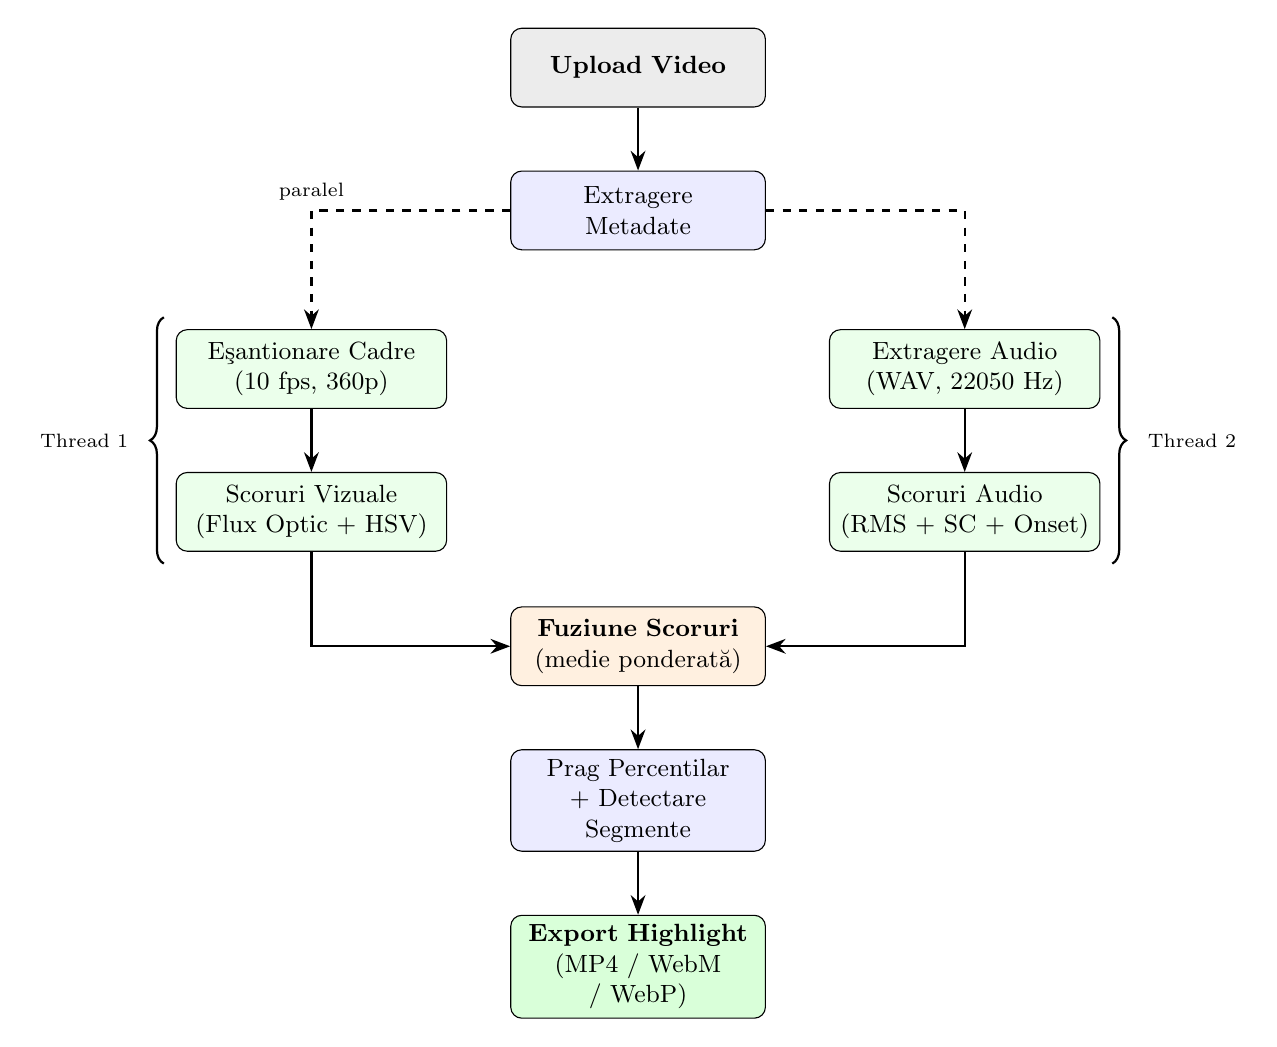
\begin{tikzpicture}[
        node distance=0.8cm and 1.2cm,
        block/.style={rectangle, draw, fill=blue!8, text width=3cm, text centered, rounded corners, minimum height=1cm, font=\small},
        bigblock/.style={rectangle, draw, fill=green!8, text width=3.2cm, text centered, rounded corners, minimum height=1cm, font=\small},
        arrow/.style={-{Stealth[length=2.5mm]}, thick},
        splitarrow/.style={-{Stealth[length=2.5mm]}, thick, dashed}
    ]
        % Row 1: Upload
        \node[block, fill=gray!15] (upload) {\textbf{Upload Video}};

        % Row 2: Metadata
        \node[block, below=of upload] (meta) {Extragere\\Metadate};

        % Row 3: Split - Visual & Audio
        \node[bigblock, below left=1cm and 0.8cm of meta] (sampling) {E\c{s}antionare Cadre\\(10 fps, 360p)};
        \node[bigblock, below right=1cm and 0.8cm of meta] (audioext) {Extragere Audio\\(WAV, 22050 Hz)};

        % Row 4: Scoring
        \node[bigblock, below=of sampling] (visual) {Scoruri Vizuale\\(Flux Optic + HSV)};
        \node[bigblock, below=of audioext] (audio) {Scoruri Audio\\(RMS + SC + Onset)};

        % Row 5: Fusion
        \node[block, fill=orange!12, below=1.2cm of $(visual)!0.5!(audio)$] (fusion) {\textbf{Fuziune Scoruri}\\(medie ponderat\u{a})};

        % Row 6: Threshold
        \node[block, below=of fusion] (thresh) {Prag Percentilar\\+ Detectare Segmente};

        % Row 7: Export
        \node[block, fill=green!15, below=of thresh] (export) {\textbf{Export Highlight}\\(MP4 / WebM / WebP)};

        % Arrows
        \draw[arrow] (upload) -- (meta);
        \draw[splitarrow] (meta) -| (sampling) node[midway, above, font=\scriptsize] {paralel};
        \draw[splitarrow] (meta) -| (audioext);
        \draw[arrow] (sampling) -- (visual);
        \draw[arrow] (audioext) -- (audio);
        \draw[arrow] (visual) |- (fusion);
        \draw[arrow] (audio) |- (fusion);
        \draw[arrow] (fusion) -- (thresh);
        \draw[arrow] (thresh) -- (export);

        % Parallel bracket annotation
        \draw[decorate, decoration={brace, amplitude=5pt, mirror}, thick]
            ($(sampling.north west)+(-0.15,0.15)$) -- ($(visual.south west)+(-0.15,-0.15)$)
            node[midway, left=8pt, font=\scriptsize, text width=1.2cm, align=center] {Thread 1};
        \draw[decorate, decoration={brace, amplitude=5pt}, thick]
            ($(audioext.north east)+(0.15,0.15)$) -- ($(audio.south east)+(0.15,-0.15)$)
            node[midway, right=8pt, font=\scriptsize, text width=1.2cm, align=center] {Thread 2};
    \end{tikzpicture}
    \caption{Arhitectura pipeline-ului de procesare a aplica\c{t}iei}
    \label{fig:pipeline}
\end{figure}

\subsection{Controlul parametrilor de c\u{a}tre utilizator}

Un aspect esen\c{t}ial al aplica\c{t}iei \^{i}l constituie posibilitatea utilizatorului de a \textbf{configura \^{i}n timp real} comportamentul algoritmului de detec\c{t}ie, direct din interfa\c{t}a grafic\u{a}, f\u{a}r\u{a}{} a necesita cuno\c{s}tin\c{t}e de programare.

\textbf{Ponderile componentelor vizual\u{a}{} \c{s}i audio} sunt controlate prin dou\u{a}{} slidere independente. Utilizatorul poate decide c\^{a}t de mult conteaz\u{a}{} mi\c{s}carea vizual\u{a}{} \c{s}i c\^{a}t de mult conteaz\u{a}{} energia sonor\u{a}{} \^{i}n decizia final\u{a}{} de selec\c{t}ie. De exemplu, pentru un meci de fotbal unde comentatorul strig\u{a}{} la fiecare faz\u{a}{} important\u{a}, se recomand\u{a}{} ponderi echilibrate (0.5/0.5). Pentru o compila\c{t}ie de scene de ac\c{t}iune dintr-un film mut, utilizatorul poate seta ponderea vizual\u{a}{} la 0.9 \c{s}i pe cea audio la 0.1. Aceste ponderi sunt normalizate intern astfel \^{i}nc\^{a}t suma lor s\u{a}{} fie \^{i}ntotdeauna egal\u{a}{} cu 1:
\begin{equation}
    F(t) = \frac{w_v}{w_v + w_a} \cdot S_{vizual}(t) + \frac{w_a}{w_v + w_a} \cdot S_{audio}(t)
\end{equation}

\textbf{Percentila de prag (Threshold Percentile)} permite utilizatorului s\u{a}{} stabileasc\u{a}{} nivelul de selectivitate. O valoare de 75 \^{i}nseamn\u{a}{} c\u{a}{} doar momentele al c\u{a}ror scor fuzionat se situeaz\u{a}{} \^{i}n primele 25\% ca intensitate vor fi incluse \^{i}n montajul final. O valoare de 90 selecteaz\u{a}{} doar primele 10\%, produc\^{a}nd un montaj mai scurt dar cu momente \c{s}i mai intense. Acest mecanism adaptiv este superior unui prag fix deoarece se calibreaz\u{a}{} automat la distribu\c{t}ia scorurilor fiec\u{a}rui videoclip \^{i}n parte.

De asemenea, utilizatorul controleaz\u{a}{} \textbf{durata minim\u{a}{} a unui clip} (pentru a evita fragmente prea scurte), \textbf{durata maxim\u{a}{} total\u{a}} a montajului final (bugetul de timp), \c{s}i \textbf{presetul de export} (Trailer 16:9, TikTok/Reel 9:16, sau Anima\c{t}ie WebP).

\subsection{Logica de fuziune a scorurilor \c{s}i detectarea segmentelor}

Dup\u{a}{} calculul independent al scorurilor vizuale \c{s}i audio, acestea trebuie combinate pe o ax\u{a}{} temporal\u{a}{} unic\u{a}. Deoarece cele dou\u{a}{} serii temporale pot avea rate de e\c{s}antionare diferite, se realizeaz\u{a}{} o \textbf{interpolare liniar\u{a}} pe o gril\u{a}{} temporal\u{a}{} comun\u{a}{} la 10\,Hz.

Scorul fuzionat $F(t)$ este supus unui \textbf{prag percentilar}. Momentele \^{i}n care $F(t)$ dep\u{a}\c{s}e\c{s}te pragul formeaz\u{a}{} segmente contigue. Algoritmul detecteaz\u{a}{} frontierele prin identificarea \textit{rising edges} \c{s}i \textit{falling edges} pe masca boolean\u{a}{} $F(t) \geq T$.

Fiec\u{a}rui segment detectat i se aplic\u{a}{} un \textbf{peak padding} de 1,5 secunde pe fiecare parte. Aceast\u{a}{} izola\c{t}ie temporal\u{a}{} simetric\u{a}{} asigur\u{a}{} captarea contextului --- de exemplu, la un gol de fotbal, algoritmul nu decupeaz\u{a}{} doar secunda exact\u{a}{} a golului, ci prinde \c{s}i construc\c{t}ia fazei \c{s}i celebrarea de la final. Segmentele care se suprapun sunt \textbf{fuzionate automat}. Dac\u{a}{} durata total\u{a}{} dep\u{a}\c{s}e\c{s}te bugetul stabilit de utilizator, se aplic\u{a}{} o \textbf{selec\c{t}ie greedy}: segmentele sunt sortate descresc\u{a}tor dup\u{a}{} scorul mediu \c{s}i sunt incluse p\^{a}n\u{a}{} la epuizarea bugetului.

\subsection{Optimiz\u{a}ri de performan\c{t}\u{a}{} \c{s}i gestiunea memoriei}

Contribu\c{t}ia tehnic\u{a}{} major\u{a}{} a acestui proiect o constituie implementarea unor optimiz\u{a}ri care permit func\c{t}ionarea aplica\c{t}iei pe hardware modest. Proiectul a fost dezvoltat \c{s}i testat pe un \textbf{laptop cu 8\,GB de memorie RAM}, o configura\c{t}ie frecvent \^{i}nt\^{a}lnit\u{a}{} \^{i}n r\^{a}ndul studen\c{t}ilor \c{s}i al creatorilor de con\c{t}inut la \^{i}nceput de drum. Aceast\u{a}{} constr\^{a}ngere a impus solu\c{t}ii ingineresti concrete:

\textbf{1. Procesare pe calupuri (Chunked Processing):} Videoclipurile HD sau 4K decomprimate \^{i}n matrice NumPy pot epuiza rapid 8\,GB de RAM. Pentru a preveni erorile de tip \textit{Out of Memory}, cadrele nu sunt stocate global. Modulul \texttt{video\_processor} utilizeaz\u{a}{} o func\c{t}ie generator (instruc\c{t}iunea Python \texttt{yield}) care produce calupuri de c\^{a}te 500 de cadre. Fiecare calup este procesat, dup\u{a}{} care matricele masive sunt eliberate din memorie prin Garbage Collection. Aceast\u{a}{} abordare de tip \textit{stream processing} limiteaz\u{a}{} consumul de memorie la un nivel constant, independent de lungimea videoclipului.

\textbf{2. Redimensionare la analiz\u{a}:} Cadrele sunt redimensionate la o \^{i}n\u{a}l\c{t}ime maxim\u{a}{} de 360 de pixeli \^{i}nainte de analiza vizual\u{a}. Calitatea detec\c{t}iei nu este afectat\u{a}{} semnificativ, dar consumul de memorie se reduce de aproximativ 9 ori pentru un videoclip Full HD (1080p).

\textbf{3. Paralelism:} Procesarea vizual\u{a}{} \c{s}i cea audio ruleaz\u{a}{} concurent pe thread-uri separate folosind \texttt{concurrent.futures.ThreadPoolExecutor}, reduc\^{a}nd timpul total la durata celei mai lente opera\c{t}iuni.

\textbf{4. Tranzi\c{t}ii pe 8 bi\c{t}i:} Efectele de fade-in \c{s}i fade-out sunt implementate printr-un filtru personalizat care opereaz\u{a}{} pe matrice de tip \texttt{uint8}, nu pe \texttt{float64} (cum face MoviePy implicit). Aceasta reduce consumul de memorie la export cu un factor de 8.

\textbf{5. Limitarea rezolu\c{t}iei la export:} Videoclipul final este limitat la maximum 720p, asigur\^{a}nd un consum echilibrat de memorie \^{i}n faza de randare.

\subsection{Crop vertical pentru social media}

Pentru presetul TikTok/Reel, aplica\c{t}ia realizeaz\u{a}{} o \textbf{t\u{a}iere centrat\u{a}} a cadrului la raportul de aspect 9:16. Algoritmul calculeaz\u{a}{} noua l\u{a}\c{t}ime $W' = H \times \frac{9}{16}$, o ajusteaz\u{a}{} la cel mai apropiat num\u{a}r par (cerin\c{t}\u{a}{} a codecurilor video), apoi extrage banda central\u{a}{} a cadrului.


% ===================== CAPITOLUL 4 =====================
\section{Utilizare \c{s}i prezentarea func\c{t}ionalit\u{a}\c{t}ii}

\subsection{Instalare \c{s}i configurare}

Aplica\c{t}ia necesit\u{a}{} \textbf{Python 3.9+} \c{s}i \textbf{FFmpeg} instalat \^{i}n PATH-ul sistemului. Pa\c{s}ii de instalare sunt:
\begin{enumerate}[noitemsep]
    \item Crearea unui mediu virtual: \texttt{python -m venv venv}
    \item Activarea mediului: \texttt{venv\textbackslash Scripts\textbackslash activate} (Windows)
    \item Instalarea dependen\c{t}elor: \texttt{pip install -r requirements.txt}
    \item Lansarea aplica\c{t}iei: \texttt{streamlit run app.py}
\end{enumerate}

Aplica\c{t}ia se deschide automat \^{i}n browser-ul implicit la adresa \texttt{http://localhost:8501}. Toate opera\c{t}iunile se desf\u{a}\c{s}oar\u{a}{} local.

\subsection{Interac\c{t}iunea cu utilizatorul}

Interfa\c{t}a a fost proiectat\u{a}{} cu scopul de a fi accesibil\u{a}{} at\^{a}t utilizatorilor tehnici, c\^{a}t \c{s}i celor f\u{a}r\u{a}{} experien\c{t}\u{a}{} \^{i}n editare video. Zona principal\u{a}{} permite \^{i}nc\u{a}rcarea fi\c{s}ierului video prin drag-and-drop (formate acceptate: MP4, AVI, MOV, MKV, WebM). Imediat dup\u{a}{} \^{i}nc\u{a}rcare, aplica\c{t}ia afi\c{s}eaz\u{a}{} metadatele videoclipului: durata, rezolu\c{t}ia, FPS-ul nativ \c{s}i num\u{a}rul total de cadre.

Bara lateral\u{a}{} (sidebar) con\c{t}ine toate controalele de configurare, organizate \^{i}n trei grupuri:

\textbf{Ponderile scorurilor} --- dou\u{a}{} slidere care permit setarea importan\c{t}ei relative a componentei vizuale \c{s}i audio. Aceast\u{a}{} func\c{t}ionalitate este deosebit de util\u{a}{} deoarece diferite tipuri de con\c{t}inut necesit\u{a}{} ponderi diferite:
\begin{itemize}[noitemsep]
    \item \textit{Meciuri de fotbal}: ponderi echilibrate (0.5 vizual, 0.5 audio) --- at\^{a}t ac\c{t}iunea de pe teren c\^{a}t \c{s}i strig\u{a}tul comentatorului sunt relevante.
    \item \textit{Scene din filme de ac\c{t}iune}: ponderea vizual\u{a}{} mai mare (0.7/0.3) --- mi\c{s}carea pe ecran este indicatorul principal.
    \item \textit{Podcasturi}: ponderea audio mai mare (0.3/0.7) --- varia\c{t}iile de voce \c{s}i ritmul conversa\c{t}iei conteaz\u{a}{} mai mult dec\^{a}t imaginea static\u{a}.
\end{itemize}

\textbf{Parametrii de detec\c{t}ie} --- percentila de prag (controlul selectivit\u{a}\c{t}ii), durata minim\u{a}{} per clip \c{s}i durata maxim\u{a}{} total\u{a}{} a montajului.

\textbf{Set\u{a}rile de export} --- presetul de proiect cu trei op\c{t}iuni: Standard Trailer (16:9 landscape), TikTok/Reel (9:16 vertical cu crop centrat), sau WebP Animation.

\begin{figure}[H]
    \centering
    \vspace{5.5cm}
    \fbox{\parbox{0.75\textwidth}{\centering\textit{[Spa\c{t}iu rezervat pentru captura de ecran cu interfa\c{t}a principal\u{a}:\\ zona de upload, metadatele video \c{s}i bara lateral\u{a}{} de configurare]}}}
    \vspace{0.3cm}
    \caption{Interfa\c{t}a principal\u{a}: zona de \^{i}nc\u{a}rcare, metadatele video \c{s}i parametrii de configurare}
    \label{fig:ui_main}
\end{figure}

\subsection{Rezultatele proces\u{a}rii}

Odat\u{a}{} finalizat\u{a}{} analiza, aplica\c{t}ia prezint\u{a}{} utilizatorului trei tipuri de rezultate:

\textbf{1. Graficul cronologic al scorurilor (Score Timeline)} --- un grafic Matplotlib care reprezint\u{a}{} vizual evolu\c{t}ia celor trei scoruri pe axa timpului. Linia turcoaz indic\u{a}{} scorul vizual (mi\c{s}care + schimb\u{a}ri de scen\u{a}), linia ro\c{s}ie indic\u{a}{} scorul audio (volum + spectru + tranzi\c{t}ii), iar linia galben\u{a}{} \^{i}ngro\c{s}at\u{a}{} reprezint\u{a}{} scorul fuzionat. Linia orizontal\u{a}{} punctat\u{a}{} traseaz\u{a}{} nivelul pragului, iar zonele umbrite vertical marcheaz\u{a}{} exact segmentele selectate. Acest grafic constituie dovada transparent\u{a}{} a modului de func\c{t}ionare al algoritmului --- utilizatorul poate \^{i}n\c{t}elege \textit{de ce} au fost alese anumite momente.

\begin{figure}[H]
    \centering
    \vspace{5cm}
    \fbox{\parbox{0.85\textwidth}{\centering\textit{[Spa\c{t}iu rezervat pentru captura de ecran cu graficul scorurilor:\\ liniile vizual/audio/fuzionat, pragul \c{s}i zonele de highlight]}}}
    \vspace{0.3cm}
    \caption{Graficul scorurilor de interes vizual \c{s}i audio pe axa timpului}
    \label{fig:timeline}
\end{figure}

\textbf{2. Lista segmentelor detectate} --- fiecare segment este afi\c{s}at ca un card cu timpul de start, timpul de final \c{s}i durata. Sunt prezentate \c{s}i metrici sumarizatoare: num\u{a}rul total de segmente, durata cumulat\u{a}{} a highlight-urilor \c{s}i procentajul de reducere a con\c{t}inutului.

\textbf{3. Previzualizarea \c{s}i desc\u{a}rcarea fi\c{s}ierului final} --- montajul generat poate fi vizualizat direct \^{i}n browser \c{s}i desc\u{a}rcat printr-un buton dedicat. Tranzi\c{t}iile dintre segmente sunt de tip fade-in/fade-out, iar fi\c{s}ierul este deja optimizat pentru distribu\c{t}ie.

\begin{figure}[H]
    \centering
    \vspace{5cm}
    \fbox{\parbox{0.75\textwidth}{\centering\textit{[Spa\c{t}iu rezervat pentru captura de ecran cu lista segmentelor detectate,\\ metricile sumarizatoare \c{s}i butonul de desc\u{a}rcare]}}}
    \vspace{0.3cm}
    \caption{Segmentele detectate, metricile de compresie \c{s}i op\c{t}iunea de desc\u{a}rcare}
    \label{fig:segments}
\end{figure}


% ===================== CAPITOLUL 5 =====================
\section{Concluzii}

Proiectul ,,Smart Video Highlight \& GIF Generator'' a demonstrat c\u{a}{} extragerea inteligent\u{a}{} a momentelor cheie din materiale multimedia poate fi realizat\u{a}{} eficient pe hardware accesibil, f\u{a}r\u{a}{} a necesita procesare \^{i}n cloud, GPU dedicat sau modele masive de Deep Learning.

Obiectivele propuse \^{i}n sec\c{t}iunea 1.2 au fost \^{i}ndeplinite integral:
\begin{itemize}[noitemsep]
    \item \textbf{Procesarea 100\% local\u{a}} a fost realizat\u{a}{} --- toate opera\c{t}iunile se desf\u{a}\c{s}oar\u{a}{} pe calculatorul utilizatorului, f\u{a}r\u{a}{} transmiterea datelor c\u{a}tre servere externe.
    \item \textbf{Func\c{t}ionarea f\u{a}r\u{a}{} GPU} a fost demonstrat\u{a}{} --- algoritmii de flux optic Farneb\"{a}ck, corela\c{t}ia histogramelor HSV \c{s}i extragerea descriptorilor audio librosa func\c{t}ioneaz\u{a}{} exclusiv pe CPU.
    \item \textbf{Compatibilitatea cu hardware modest} a fost validat\u{a}{} prin dezvoltarea \c{s}i testarea integral\u{a}{} pe un laptop cu 8\,GB de RAM, gra\c{t}ie sistemului de chunked processing \c{s}i a optimiz\u{a}rilor de memorie descrise \^{i}n sec\c{t}iunea 3.5.
    \item \textbf{Controlul granular} este asigurat prin slidere intuitive pentru ponderile vizual/audio \c{s}i pentru percentila de prag, permi\c{t}\^{a}nd utilizatorului s\u{a}{} adapteze algoritmul la tipul de con\c{t}inut procesat.
    \item \textbf{Exportul configurabil} pentru social media func\c{t}ioneaz\u{a}{} corect at\^{a}t \^{i}n format landscape 16:9 c\^{a}t \c{s}i \^{i}n format vertical 9:16 cu crop centrat.
\end{itemize}

Fa\c{t}\u{a}{} de solu\c{t}iile comerciale analizate \^{i}n sec\c{t}iunea 2.1, aplica\c{t}ia prezint\u{a}{} avantajul unic al \textbf{transparen\c{t}ei algoritmice}: graficul timeline permite utilizatorului s\u{a}{} \^{i}n\c{t}eleag\u{a}{} exact cum au fost selectate momentele de interes, spre deosebire de instrumentele ,,black-box'' care nu ofer\u{a}{} explica\c{t}ii ale deciziilor lor.

Ca \textbf{limit\u{a}ri}, aplica\c{t}ia nu realizeaz\u{a}{} recunoa\c{s}tere semantic\u{a}{} a con\c{t}inutului (nu ,,\^{i}n\c{t}elege'' ce se \^{i}nt\^{a}mpl\u{a}{} pe ecran, ci detecteaz\u{a}{} doar mi\c{s}carea \c{s}i sunetul). De asemenea, calitatea detec\c{t}iei depinde de calitatea pistei audio --- un videoclip cu fundal muzical uniform va produce scoruri audio mai pu\c{t}in diferen\c{t}iate.

Ca \textbf{direc\c{t}ii viitoare}, se pot integra: recunoa\c{s}terea textului de pe ecran (OCR) pentru identificarea scorului unui meci direct din graficele afi\c{s}ate, identificarea automat\u{a}{} a vorbitorului activ (Speaker Diarization) pentru podcasturi cu mai mul\c{t}i participan\c{t}i, \c{s}i exportul direct pe platformele de social media prin API-urile acestora.

\^{I}n concluzie, proiectul r\u{a}spunde unei nevoi reale a comunit\u{a}\c{t}ii de creatori de con\c{t}inut short-form video, oferind un instrument practic, transparent \c{s}i accesibil financiar, care reduce semnificativ timpul necesar procesului de editare.


% ===================== DECLARATIE LLM =====================
\vspace{0.8cm}
\noindent\textbf{Declara\c{t}ie privind utilizarea modelelor de limbaj (LLM)}

\noindent \^{I}n conformitate cu Regulamentul Universit\u{a}\c{t}ii Politehnica din Bucure\c{s}ti, declar c\u{a}{} am utilizat un model de limbaj de tip LLM (Large Language Model) \^{i}n urm\u{a}toarele scopuri limitate:
\begin{itemize}[noitemsep]
    \item \textbf{Stilizarea CSS} a interfe\c{t}ei Streamlit --- generarea regulilor de stil vizual (culori, gradien\c{t}i, umbre) pentru componentele UI din fi\c{s}ierul \texttt{app.py}.
    \item \textbf{Configurarea mediului de execu\c{t}ie} --- asistare la crearea structurii de mediu virtual Python (\textit{virtual environment}), a fi\c{s}ierului \texttt{requirements.txt} \c{s}i a scriptului de lansare \texttt{start\_app.bat}.
    \item \textbf{Planificarea ini\c{t}ial\u{a}} --- realizarea unui plan preliminar al structurii proiectului pentru a stabili arhitectura modular\u{a}{} \c{s}i fluxul de procesare.
\end{itemize}

\noindent Logica de baz\u{a}{} a aplica\c{t}iei, implementarea algoritmilor de procesare vizual\u{a}{} (flux optic, histograme HSV), a descriptorilor audio (RMS, centroid spectral, onset strength), a mecanismului de fuziune a scorurilor, a optimiz\u{a}rilor de memorie (chunked processing, fade uint8) \c{s}i a pipeline-ului complet de procesare reprezint\u{a}{} contribu\c{t}ia mea individual\u{a}.


% ===================== BIBLIOGRAFIE =====================
\newpage
\begin{thebibliography}{99}

\bibitem{opencv2000}
G. Bradski (2000), \emph{The OpenCV Library}, Dr. Dobb's Journal of Software Tools.

\bibitem{farneback2003}
G. Farneb{\"a}ck (2003), \emph{Two-Frame Motion Estimation Based on Polynomial Expansion}, Proceedings of the 13th Scandinavian Conference on Image Analysis (SCIA), pp. 363--370.

\bibitem{itu2003}
ITU-T Recommendation H.264 (2003), \emph{Advanced Video Coding for Generic Audiovisual Services}, International Telecommunication Union.

\bibitem{librosa2015}
B. McFee, C. Raffel, D. Liang, D. P. W. Ellis, M. McVicar, E. Battenberg, O. Nieto (2015), \emph{librosa: Audio and Music Signal Analysis in Python}, Proceedings of the 14th Python in Science Conference, pp. 18--24.

\bibitem{moviepy2015}
Zulko et al. (2015), \emph{MoviePy: Video editing with Python}. \url{https://zulko.github.io/moviepy/} (Accesat \^{i}n aprilie 2026).

\bibitem{muller2016}
A. C. M{\"u}ller, S. Guido (2016), \emph{Introduction to Machine Learning with Python: A Guide for Data Scientists}, O'Reilly Media, ISBN: 978-1-449-36941-5.

\bibitem{cisco2020}
Cisco Systems (2020), \emph{Cisco Annual Internet Report (2018--2023)}, White Paper, \url{https://www.cisco.com/c/en/us/solutions/collateral/executive-perspectives/annual-internet-report/white-paper-c11-741490.html} (Accesat \^{i}n aprilie 2026).

\bibitem{adobe2026}
Adobe Inc. (Accesat \^{i}n aprilie 2026), \emph{Auto Reframe --- Premiere Pro User Guide}, \url{https://helpx.adobe.com/premiere-pro/using/auto-reframe.html}.

\bibitem{opusclip2026}
OpusClip (Accesat \^{i}n aprilie 2026), \emph{AI Video Repurposing Platform}, \url{https://www.opus.pro/}.

\bibitem{capcut2026}
CapCut --- ByteDance (Accesat \^{i}n aprilie 2026), \emph{CapCut Video Editor}, \url{https://www.capcut.com/}.

\bibitem{gling2026}
Gling (Accesat \^{i}n aprilie 2026), \emph{AI Video Editing for Content Creators}, \url{https://www.gling.ai/}.

\bibitem{streamlit2026}
Streamlit Inc. (Accesat \^{i}n aprilie 2026), \emph{Streamlit --- A faster way to build and share data apps}, \url{https://docs.streamlit.io/}.

\end{thebibliography}

\end{document}
